\documentclass[11pt]{article}
\usepackage[margin=2.2cm]{geometry}
\usepackage{booktabs}
\usepackage{threeparttable}
\usepackage{amsmath}
\usepackage{graphicx}
\begin{document}

\begin{table}[htbp]
\centering
\begin{threeparttable}
\caption{Air connectivity and aviation CO$_2$: main results}
\label{tab:main}
\footnotesize
\begin{tabular}{lcccccc}
\toprule
 & \multicolumn{1}{c}{Bunker CO$_2$} & \multicolumn{1}{c}{LTO CO$_2$} & \multicolumn{1}{c}{50/50 CO$_2$} & \multicolumn{1}{c}{Intl.\ CO$_2$} & \multicolumn{1}{c}{Seat-km} & \multicolumn{1}{c}{Intensity} \\
 & (1) & (2) & (3) & (4) & (5) & (6) \\
\midrule
\multicolumn{7}{l}{\textit{Panel A. OLS}} \\
  ln GACI (cwm) & 3.585$^{***}$ & 3.043$^{***}$ & 3.566$^{***}$ & 3.874$^{***}$ & 3.941$^{***}$ & -0.355$^{***}$ \\
   & (0.175) & (0.177) & (0.175) & (0.198) & (0.183) & (0.043) \\
  $N$ & 4,634 & 4,634 & 4,634 & 4,633 & 4,634 & 4,634 \\
\midrule
\multicolumn{7}{l}{\textit{Panel B. 2SLS, Feyrer instrument, capacity-weighted mean}} \\
  ln GACI (cwm) & 5.669$^{***}$ & 5.921$^{***}$ & 5.620$^{***}$ & 5.690$^{***}$ & 6.068$^{***}$ & -0.399$^{***}$ \\
   & (0.412) & (0.448) & (0.409) & (0.415) & (0.443) & (0.118) \\
  KP $F$ & 153.6 & 153.6 & 153.6 & 152.7 & 153.6 & 153.6 \\
  $N$ & 4,634 & 4,634 & 4,634 & 4,633 & 4,634 & 4,634 \\
\midrule
\multicolumn{7}{l}{\textit{Panel C. 2SLS, GACI sum}} \\
  ln GACI (sum) & 2.283$^{***}$ & 2.384$^{***}$ & 2.263$^{***}$ & 2.291$^{***}$ & 2.443$^{***}$ & -0.161$^{***}$ \\
   & (0.224) & (0.219) & (0.222) & (0.237) & (0.250) & (0.052) \\
  KP $F$ & 90.3 & 90.3 & 90.3 & 89.5 & 90.3 & 90.3 \\
  $N$ & 4,634 & 4,634 & 4,634 & 4,633 & 4,634 & 4,634 \\
\midrule
\multicolumn{7}{l}{\textit{Panel D. 2SLS, GACI max}} \\
  ln GACI (max) & 4.822$^{***}$ & 5.036$^{***}$ & 4.780$^{***}$ & 4.836$^{***}$ & 5.161$^{***}$ & -0.340$^{***}$ \\
   & (0.329) & (0.348) & (0.327) & (0.343) & (0.361) & (0.101) \\
  KP $F$ & 172.0 & 172.0 & 172.0 & 171.0 & 172.0 & 172.0 \\
  $N$ & 4,634 & 4,634 & 4,634 & 4,633 & 4,634 & 4,634 \\
\midrule
\multicolumn{7}{l}{\textit{Panel E. 2SLS, GACI mean}} \\
  ln GACI (mean) & 5.897$^{***}$ & 6.159$^{***}$ & 5.846$^{***}$ & 5.902$^{***}$ & 6.313$^{***}$ & -0.415$^{***}$ \\
   & (0.591) & (0.623) & (0.587) & (0.593) & (0.624) & (0.122) \\
  KP $F$ & 136.2 & 136.2 & 136.2 & 135.6 & 136.2 & 136.2 \\
  $N$ & 4,634 & 4,634 & 4,634 & 4,633 & 4,634 & 4,634 \\
\bottomrule
\end{tabular}
\begin{tablenotes}[flushleft]
\footnotesize
\item Notes: Country-year panel, 1996--2023. All specifications include country and year fixed effects and control for log population and log sea market access. Outcomes are in logs: total aviation CO$_2$ under the bunker convention (all cruise plus departure-side LTO assigned to the departure country), landing-and-take-off CO$_2$ only, CO$_2$ with cruise split 50/50 between endpoint countries, bunker CO$_2$ from international flights, scheduled departing seat-kilometres, and CO$_2$ per seat-km. The instrument in Panels B--E interacts world aviation technology with air-versus-sea geography (Feyrer-type). Robust standard errors in parentheses. $^{***}$, $^{**}$, $^{*}$: significance at 1, 5, and 10 percent.
\end{tablenotes}
\end{threeparttable}
\end{table}

\begin{table}[htbp]
\centering
\begin{threeparttable}
\caption{Connectivity spillovers: neighbouring countries' connectivity and own aviation outcomes}
\label{tab:spillover}
\footnotesize
\begin{tabular}{lccccc}
\toprule
\multicolumn{6}{l}{\textit{Panel A. 2SLS: neighbour connectivity instrumented}} \\
 & \multicolumn{1}{c}{Bunker CO$_2$} & \multicolumn{1}{c}{Intl.\ CO$_2$} & \multicolumn{1}{c}{Intensity} & \multicolumn{1}{c}{Trade volume} & \\
 & (1) & (2) & (3) & (4) & \\
\midrule
  ln neighbour GACI & 7.454$^{***}$ & 10.237$^{***}$ & 1.312$^{**}$ & 2.072 & \\
   & (1.994) & (2.092) & (0.534) & (2.011) & \\
  Own Feyrer shifter & 0.254$^{**}$ & 0.076 & -0.134$^{***}$ & 0.157 & \\
   & (0.122) & (0.128) & (0.037) & (0.124) & \\
  KP $F$ & 134.1 & 134.0 & 134.1 & 134.1 & \\
  $N$ & 4,623 & 4,622 & 4,623 & 4,623 & \\
\midrule
\multicolumn{6}{l}{\textit{Panel B. Margins of the own response to neighbour connectivity (same specification)}} \\
 & \multicolumn{1}{c}{Flights} & \multicolumn{1}{c}{Seat-km} & \multicolumn{1}{c}{Aircraft size} & \multicolumn{1}{c}{Stage length} & \multicolumn{1}{c}{Intl.\ share} \\
 & (1) & (2) & (3) & (4) & (5) \\
\midrule
  ln neighbour GACI & 2.730 & 6.141$^{***}$ & 5.437$^{***}$ & -2.026$^{**}$ & 1.046$^{***}$ \\
   & (2.216) & (2.083) & (1.170) & (1.008) & (0.281) \\
\bottomrule
\end{tabular}
\begin{tablenotes}[flushleft]
\footnotesize
\item Notes: Neighbour connectivity is the inverse-distance-weighted average of all other countries' log GACI (capacity-weighted mean), with weights based on haversine distances between countries' aviation activity centroids. It is instrumented by the identically weighted average of other countries' Feyrer shifters; the own Feyrer shifter enters directly, so the own-connectivity effect is in reduced form. Own and neighbour connectivity cannot be jointly instrumented because the two shifters are collinear within country. All specifications include country and year fixed effects and control for log population and log sea market access. Robust standard errors in parentheses. $^{***}$, $^{**}$, $^{*}$: significance at 1, 5, and 10 percent.
\end{tablenotes}
\end{threeparttable}
\end{table}

\begin{table}[htbp]
\centering
\begin{threeparttable}
\caption{Causal mediation of the connectivity effect on aviation CO$_2$}
\label{tab:mediation}
\footnotesize
\begin{tabular}{lccccc}
\toprule
\multicolumn{6}{l}{\textit{Panel A. Instrumental-variable product of coefficients (2SLS scale; total effect 5.669)}} \\
Mediator & $a$: GACI$\rightarrow M$ & $b$: $M\rightarrow$CO$_2$ & ACME ($a\times b$) & Sobel $p$ & Share mediated \\
\midrule
  Flight frequency & 6.976 & 0.682 & 4.756 & 0.000 & 83.9\% \\
  Seat-kilometres & 6.068 & 0.808 & 4.901 & 0.000 & 86.5\% \\
  International share & 0.096 & -1.060 & -0.102 & 0.060 & -1.8\% \\
\midrule
\multicolumn{6}{l}{\textit{Panel B. Imai, Keele and Yamamoto (2010) mediation (OLS scale; total effect 3.582)}} \\
Mediator & ACME & Direct effect & Total effect & & Share mediated \\
\midrule
  Flight frequency & 1.766 & 1.816 & 3.582 & & 49.3\% \\
  Seat-kilometres & 3.424 & 0.159 & 3.583 & & 95.6\% \\
  International share & -0.077 & 3.657 & 3.580 & & -2.1\% \\
\bottomrule
\end{tabular}
\begin{tablenotes}[flushleft]
\footnotesize
\item Notes: Outcome is log total bunker CO$_2$; the treatment is log GACI (capacity-weighted mean). Panel A instruments the treatment with the Feyrer shifter in each equation and combines the paths by the product method with delta-method (Sobel) standard errors. Panel B implements the algorithm of Imai, Keele and Yamamoto (2010) by quasi-Bayesian simulation (200 draws) on least-squares models with country and year indicator variables. Each row is a separate single-mediator analysis and the mediators overlap, so shares do not sum across rows. All models control for log population and log sea market access. Sequential ignorability of the mediator is assumed conditional on the fixed effects.
\end{tablenotes}
\end{threeparttable}
\end{table}

\begin{table}[htbp]
\centering
\begin{threeparttable}
\caption{Heterogeneity of the connectivity elasticity}
\label{tab:hetero}
\footnotesize
\begin{tabular}{lcccc}
\toprule
 & Coefficient & s.e. & KP $F$ & $N$ \\
\midrule
\multicolumn{5}{l}{\textit{Panel A. Total CO$_2$ by baseline income tercile}} \\
  Low income & 11.431$^{***}$ & (1.338) & 35.2 & 1,595 \\
  Middle income & 5.906$^{***}$ & (0.782) & 48.2 & 1,547 \\
  High income & 0.350 & (1.106) & 10.1 & 1,491 \\
\midrule
\multicolumn{5}{l}{\textit{Panel B. Total CO$_2$ by baseline connectivity tercile}} \\
  Low connectivity & 9.018$^{***}$ & (0.656) & 117.4 & 1,452 \\
  Middle connectivity & 5.642$^{***}$ & (0.908) & 29.9 & 1,526 \\
  High connectivity & 0.452 & (2.201) & 1.8 & 1,655 \\
\midrule
\multicolumn{5}{l}{\textit{Panel C. Total CO$_2$ by region}} \\
  Europe & 0.236 & (0.616) & 55.5 & 1,189 \\
  Asia--Pacific & 5.424$^{***}$ & (0.667) & 64.4 & 1,110 \\
  Africa & 8.385$^{***}$ & (1.688) & 20.2 & 1,230 \\
  Latin America & 3.229$^{***}$ & (0.900) & 14.1 & 683 \\
  Middle East & \multicolumn{4}{c}{not identified (KP $F<2$)} \\
  North America & \multicolumn{4}{c}{not identified (KP $F<2$)} \\
\midrule
\multicolumn{5}{l}{\textit{Panel D. Intensity by baseline income tercile}} \\
  Low income & -1.057$^{***}$ & (0.299) & 35.5 & 1,596 \\
  Middle income & -0.372 & (0.241) & 48.2 & 1,547 \\
  High income & 1.012 & (0.715) & 10.1 & 1,491 \\
\bottomrule
\end{tabular}
\begin{tablenotes}[flushleft]
\footnotesize
\item Notes: Split-sample 2SLS with the Feyrer instrument; terciles are formed on 1996 values. All specifications include country and year fixed effects and control for log population and log sea market access. The Middle East and North America cells have too little instrument variation for inference. Robust standard errors in parentheses. $^{***}$, $^{**}$, $^{*}$: significance at 1, 5, and 10 percent.
\end{tablenotes}
\end{threeparttable}
\end{table}

\begin{table}[htbp]
\centering
\begin{threeparttable}
\caption{Temporal split of the connectivity elasticity}
\label{tab:temporal}
\footnotesize
\begin{tabular}{lcccc}
\toprule
 & \multicolumn{1}{c}{Bunker CO$_2$} & \multicolumn{1}{c}{Intl.\ CO$_2$} & \multicolumn{1}{c}{Seat-km} & \multicolumn{1}{c}{Intensity} \\
 & (1) & (2) & (3) & (4) \\
\midrule
\multicolumn{5}{l}{\textit{Panel A. Full sample, 1996--2023}} \\
  ln GACI (cwm) & 5.669$^{***}$ & 5.690$^{***}$ & 6.068$^{***}$ & -0.399$^{***}$ \\
   & (0.412) & (0.415) & (0.443) & (0.118) \\
  KP $F$ & 153.6 & 152.7 & 153.6 & 153.6 \\
  $N$ & 4,634 & 4,633 & 4,634 & 4,634 \\
\midrule
\multicolumn{5}{l}{\textit{Panel B. Network-expansion era, 1996--2007}} \\
  ln GACI (cwm) & 5.613$^{***}$ & 5.809$^{***}$ & 4.837$^{***}$ & 0.776$^{***}$ \\
   & (0.665) & (0.704) & (0.626) & (0.249) \\
  KP $F$ & 75.0 & 74.9 & 75.0 & 75.0 \\
  $N$ & 1,883 & 1,882 & 1,883 & 1,883 \\
\midrule
\multicolumn{5}{l}{\textit{Panel C. Mature-network era, 2010--2023 (excl.\ 2020--2021)}} \\
  ln GACI (cwm) & 3.005$^{***}$ & 2.965$^{***}$ & 3.984$^{***}$ & -0.979$^{***}$ \\
   & (0.635) & (0.610) & (0.668) & (0.248) \\
  KP $F$ & 36.7 & 36.7 & 36.7 & 36.7 \\
  $N$ & 2,065 & 2,065 & 2,065 & 2,065 \\
\midrule
\multicolumn{5}{l}{\textit{Panel D. Unrestricted split: 1996--2009}} \\
  ln GACI (cwm) & 6.109$^{***}$ & 6.262$^{***}$ & 5.537$^{***}$ & 0.571$^{***}$ \\
   & (0.565) & (0.590) & (0.534) & (0.192) \\
  KP $F$ & 127.7 & 126.9 & 127.7 & 127.7 \\
  $N$ & 2,218 & 2,217 & 2,218 & 2,218 \\
\midrule
\multicolumn{5}{l}{\textit{Panel E. Unrestricted split: 2010--2023 (weak first stage)}} \\
  ln GACI (cwm) & 1.213 & 1.051 & 1.829 & -0.617 \\
   & (1.394) & (1.463) & (1.598) & (0.739) \\
  KP $F$ & 7.0 & 7.0 & 7.0 & 7.0 \\
  $N$ & 2,415 & 2,415 & 2,415 & 2,415 \\
\bottomrule
\end{tabular}
\begin{tablenotes}[flushleft]
\footnotesize
\item Notes: 2SLS with the Feyrer instrument; specifications as in Table~\ref{tab:main}. Panels B and C split the sample at its midpoint (2010) and exclude the crisis years: Panel B ends before the global financial crisis (2008--2009) and Panel C drops the COVID-19 collapse (2020--2021). Both subperiods are strongly identified and the elasticity in each is above one; the pre-versus-post difference for total CO$_2$ is 2.61 ($p = 0.005$). Panels D and E report the unrestricted split for reference: the weak first stage in Panel E (KP $F = 7.0$) is driven by the COVID years, whose exclusion in Panel C restores $F$ to 36.7, so the small point estimates in Panel E reflect a contaminated first stage rather than a vanished effect. Robust standard errors in parentheses. $^{***}$, $^{**}$, $^{*}$: significance at 1, 5, and 10 percent.
\end{tablenotes}
\end{threeparttable}
\end{table}

\clearpage
\begin{figure}[htbp]
\centering
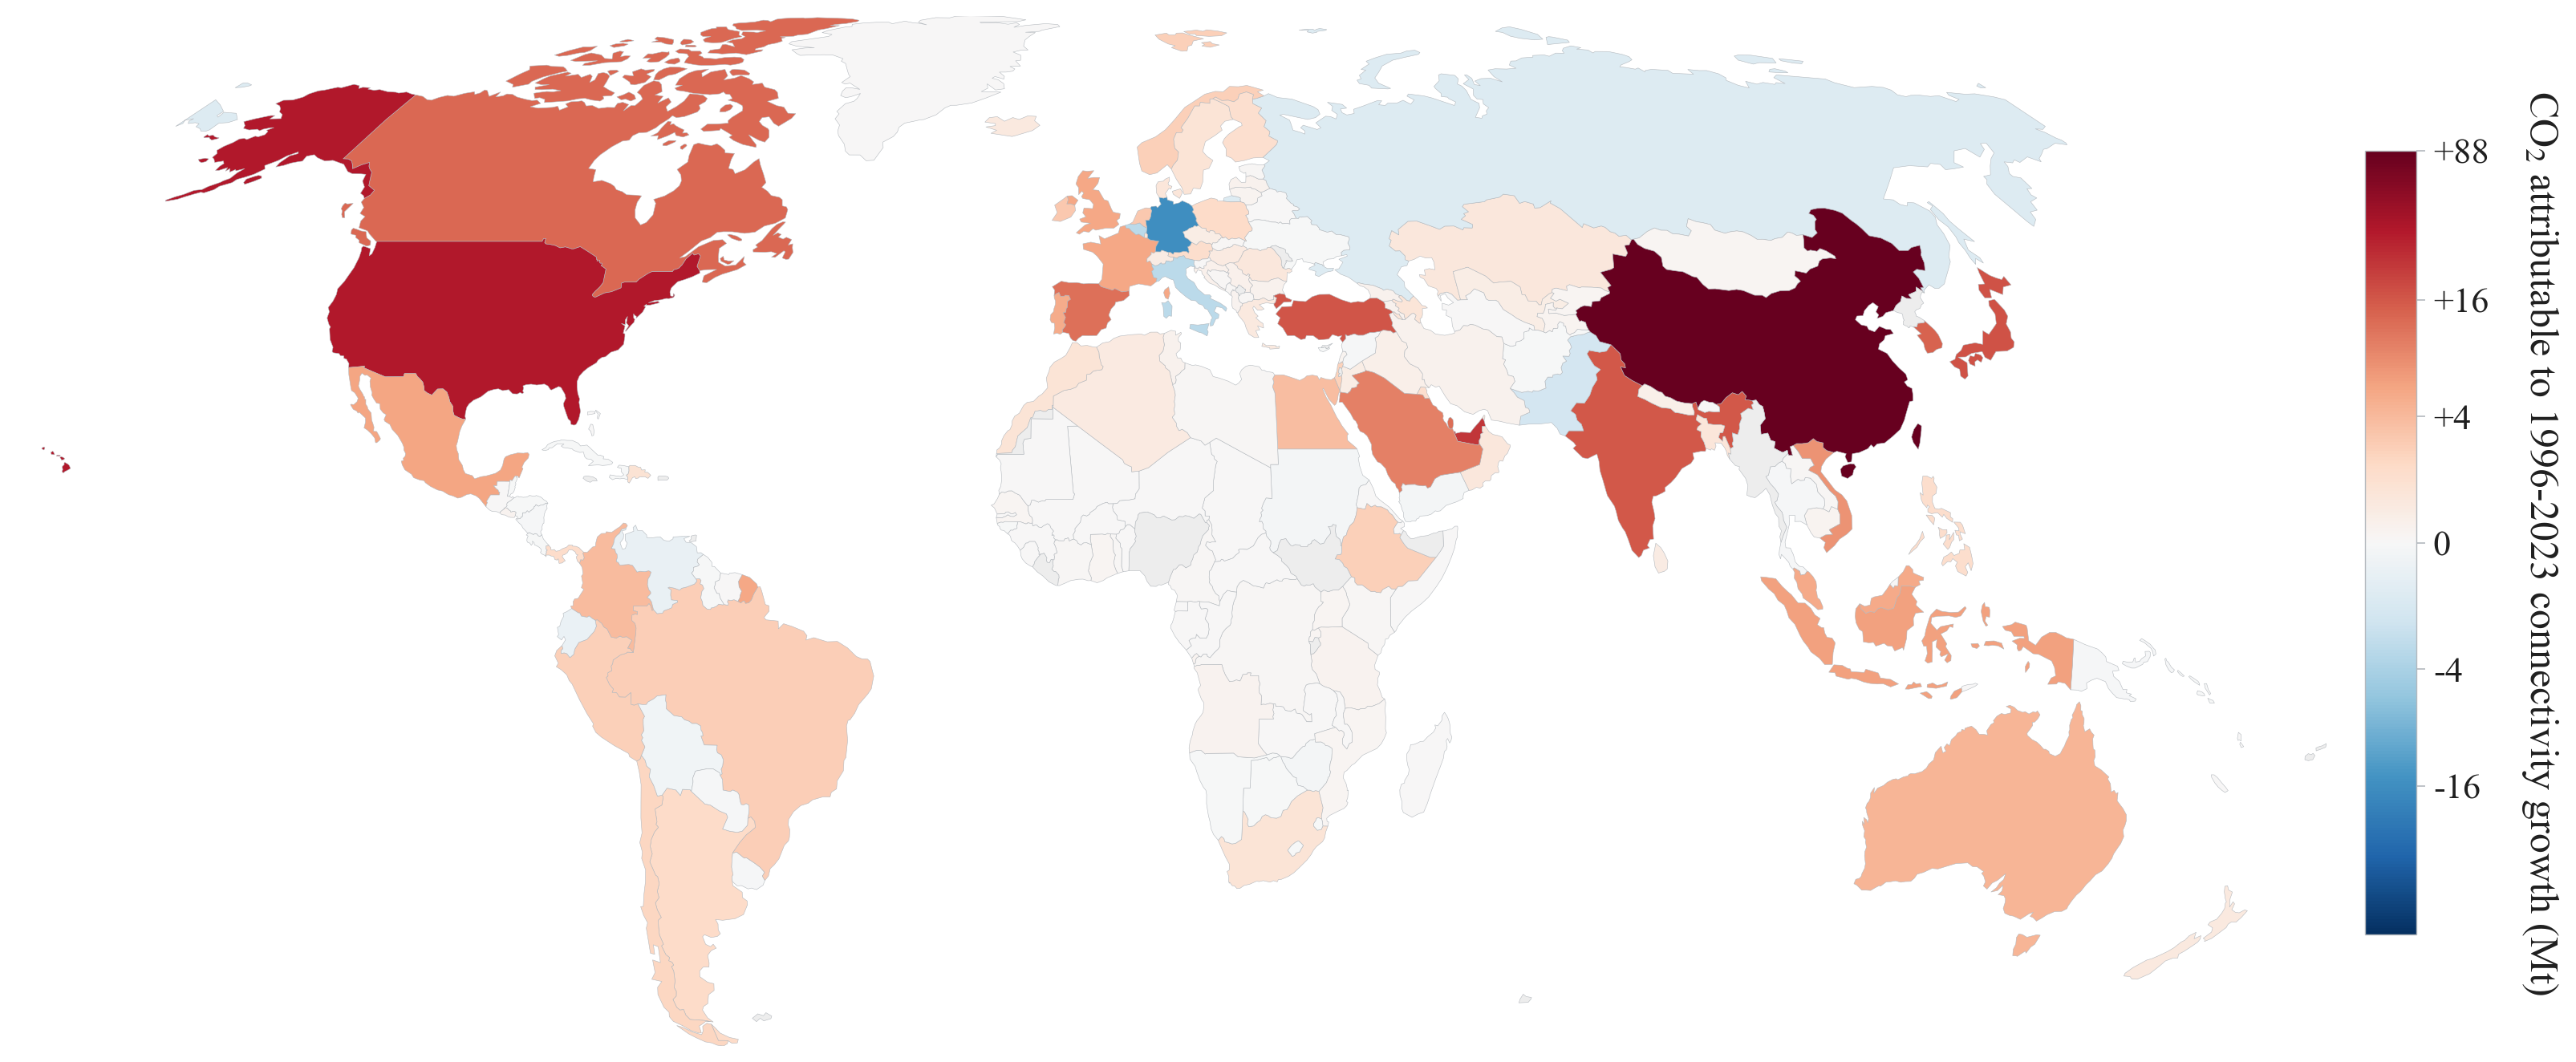
\includegraphics[width=0.92\textwidth]{CO2_map_attributed_2023.png}
\caption{Aviation CO$_2$ attributed to post-1996 connectivity growth, 2023 (Mt). White denotes zero; the attribution applies the Feyrer-instrument elasticity to each country's connectivity change.}
\label{fig:attributed}
\end{figure}

\begin{figure}[htbp]
\centering
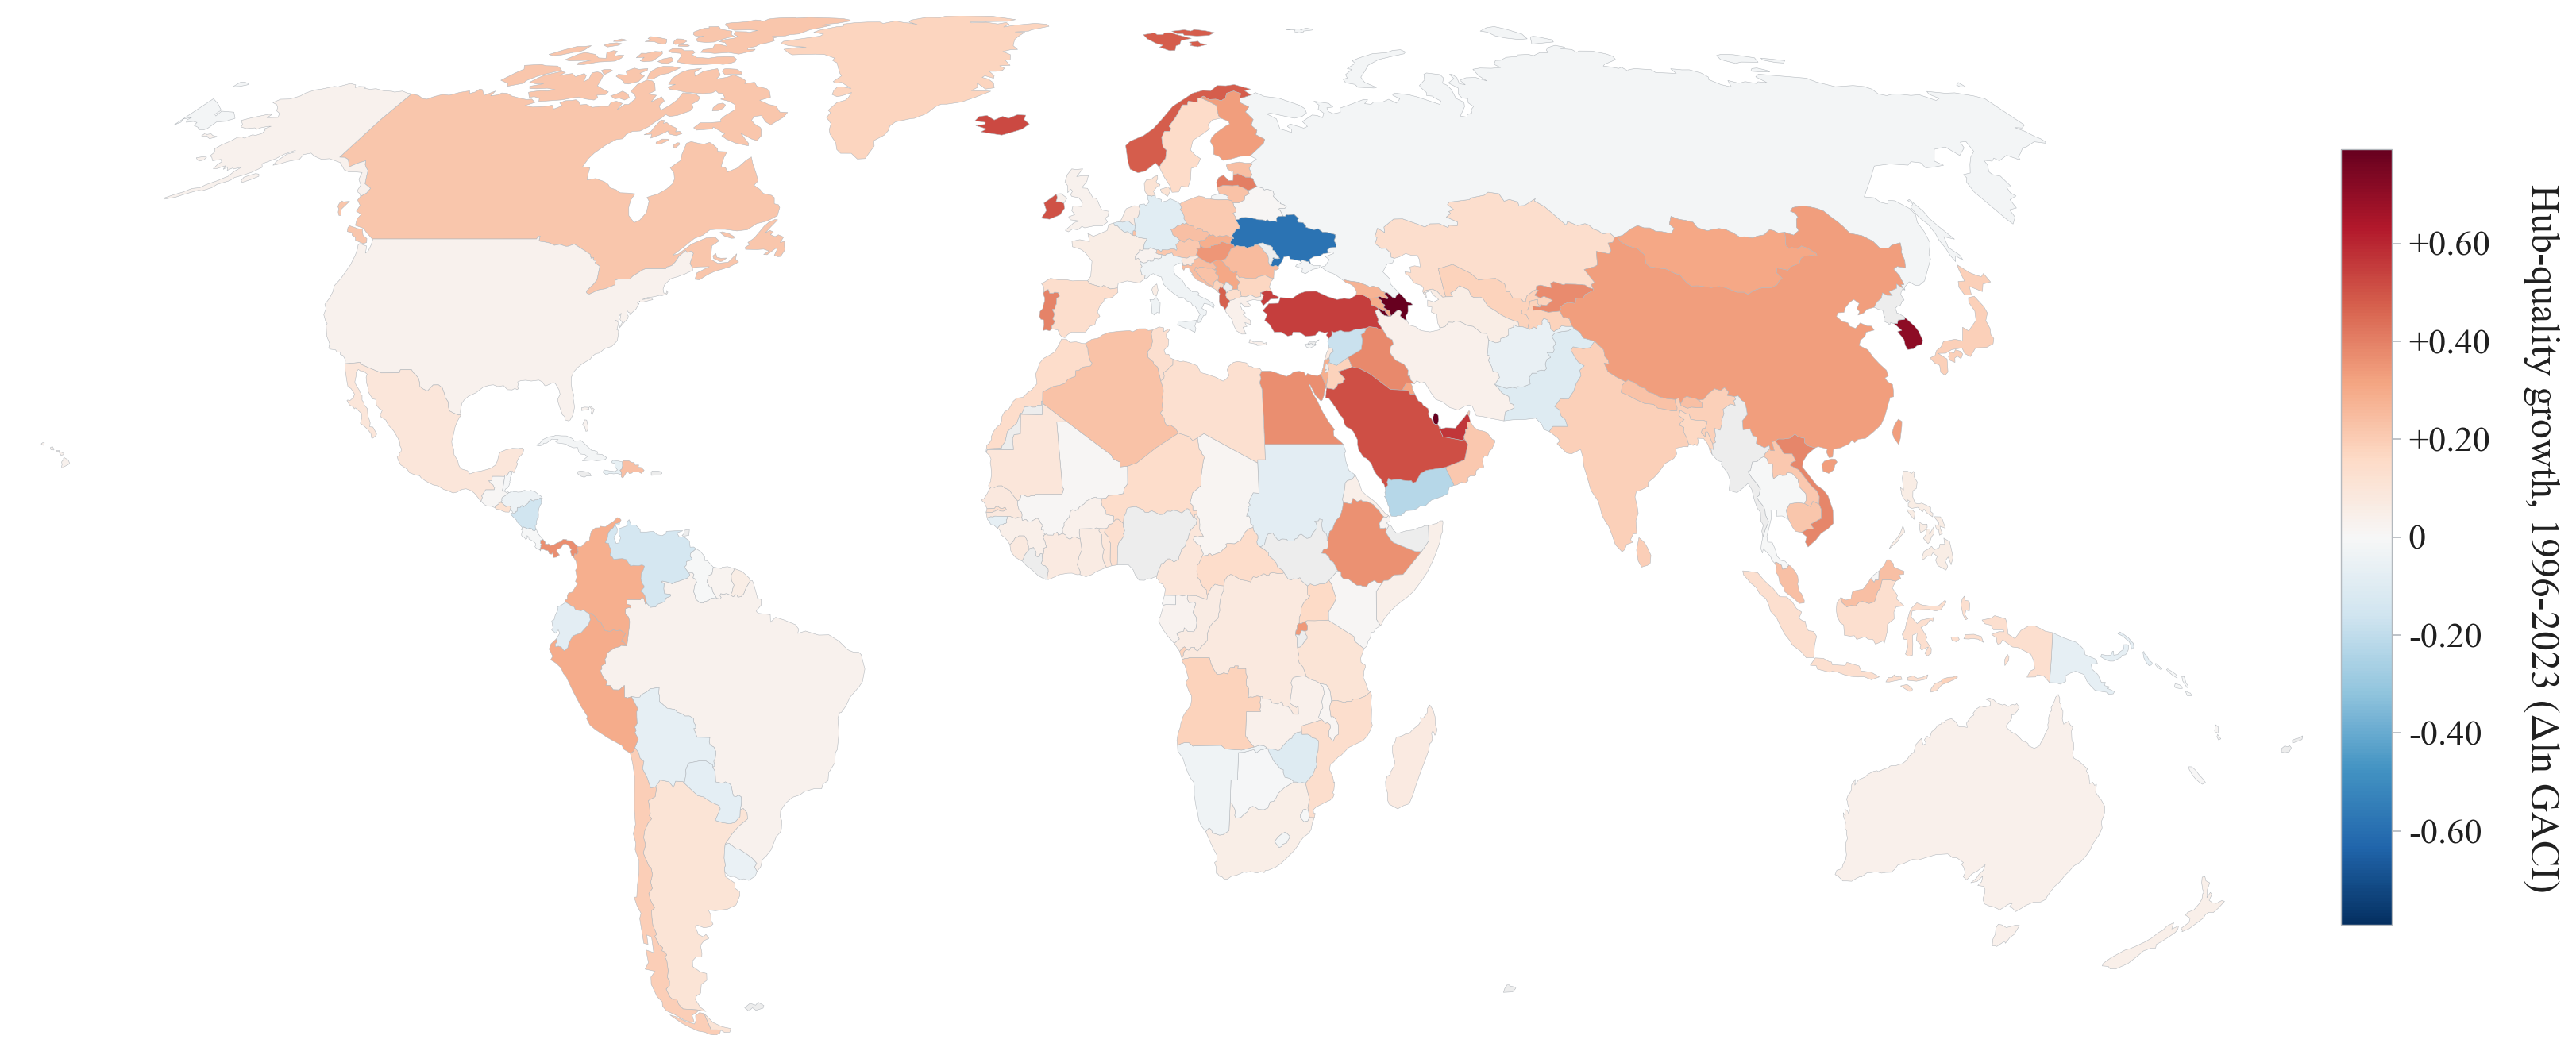
\includegraphics[width=0.92\textwidth]{CO2_map_dlngaci.png}
\caption{Change in log air connectivity (GACI, capacity-weighted mean), 1996--2023.}
\label{fig:dlngaci}
\end{figure}

\begin{figure}[htbp]
\centering
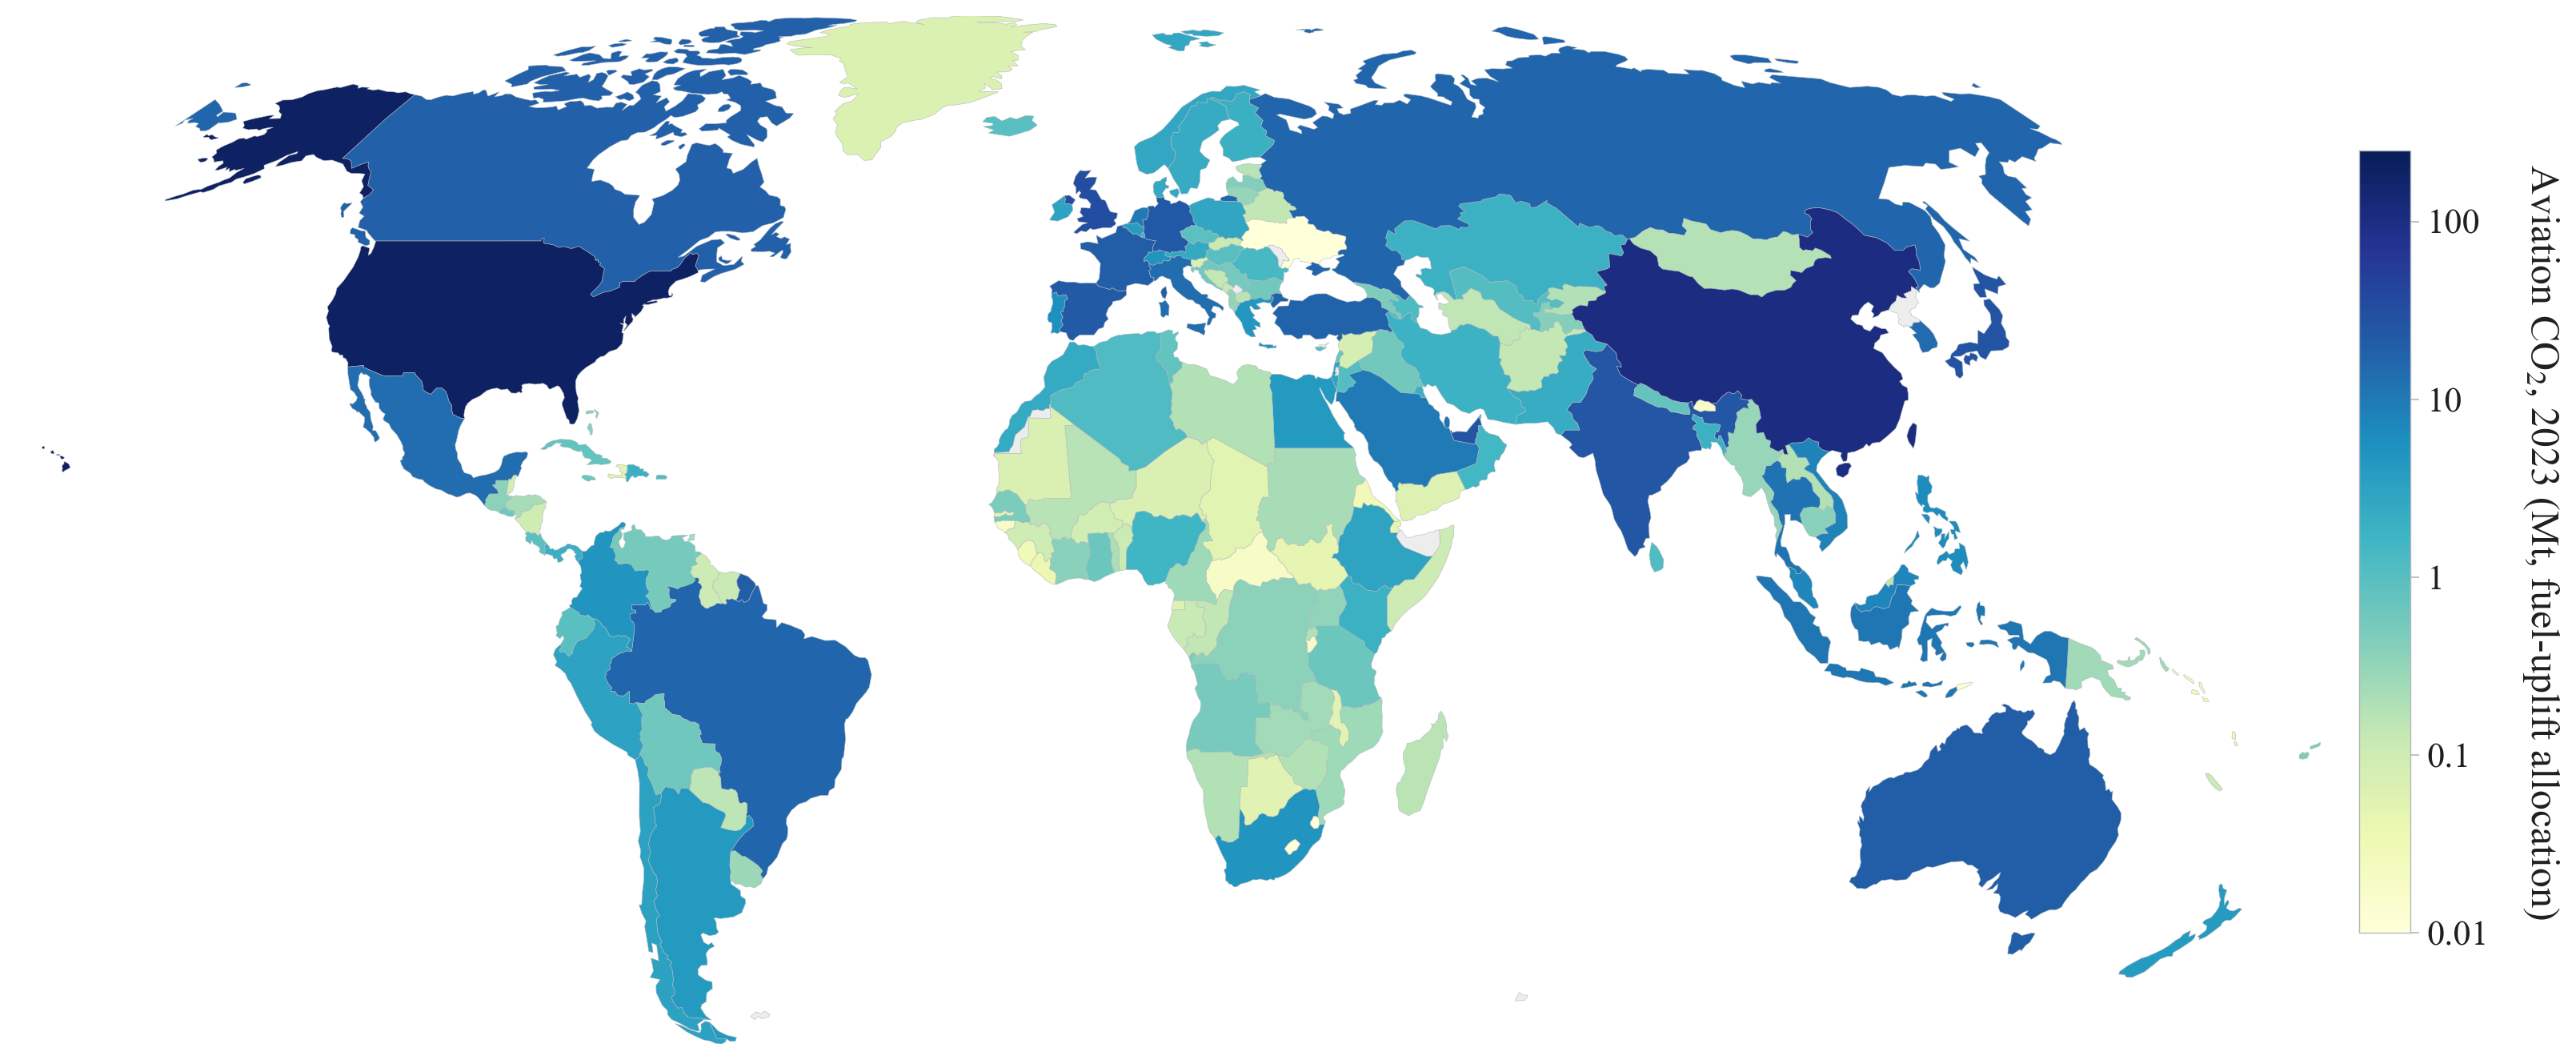
\includegraphics[width=0.92\textwidth]{CO2_map_levels_2023.png}
\caption{Aviation CO$_2$ levels under the bunker convention, 2023.}
\label{fig:levels}
\end{figure}

\begin{figure}[htbp]
\centering
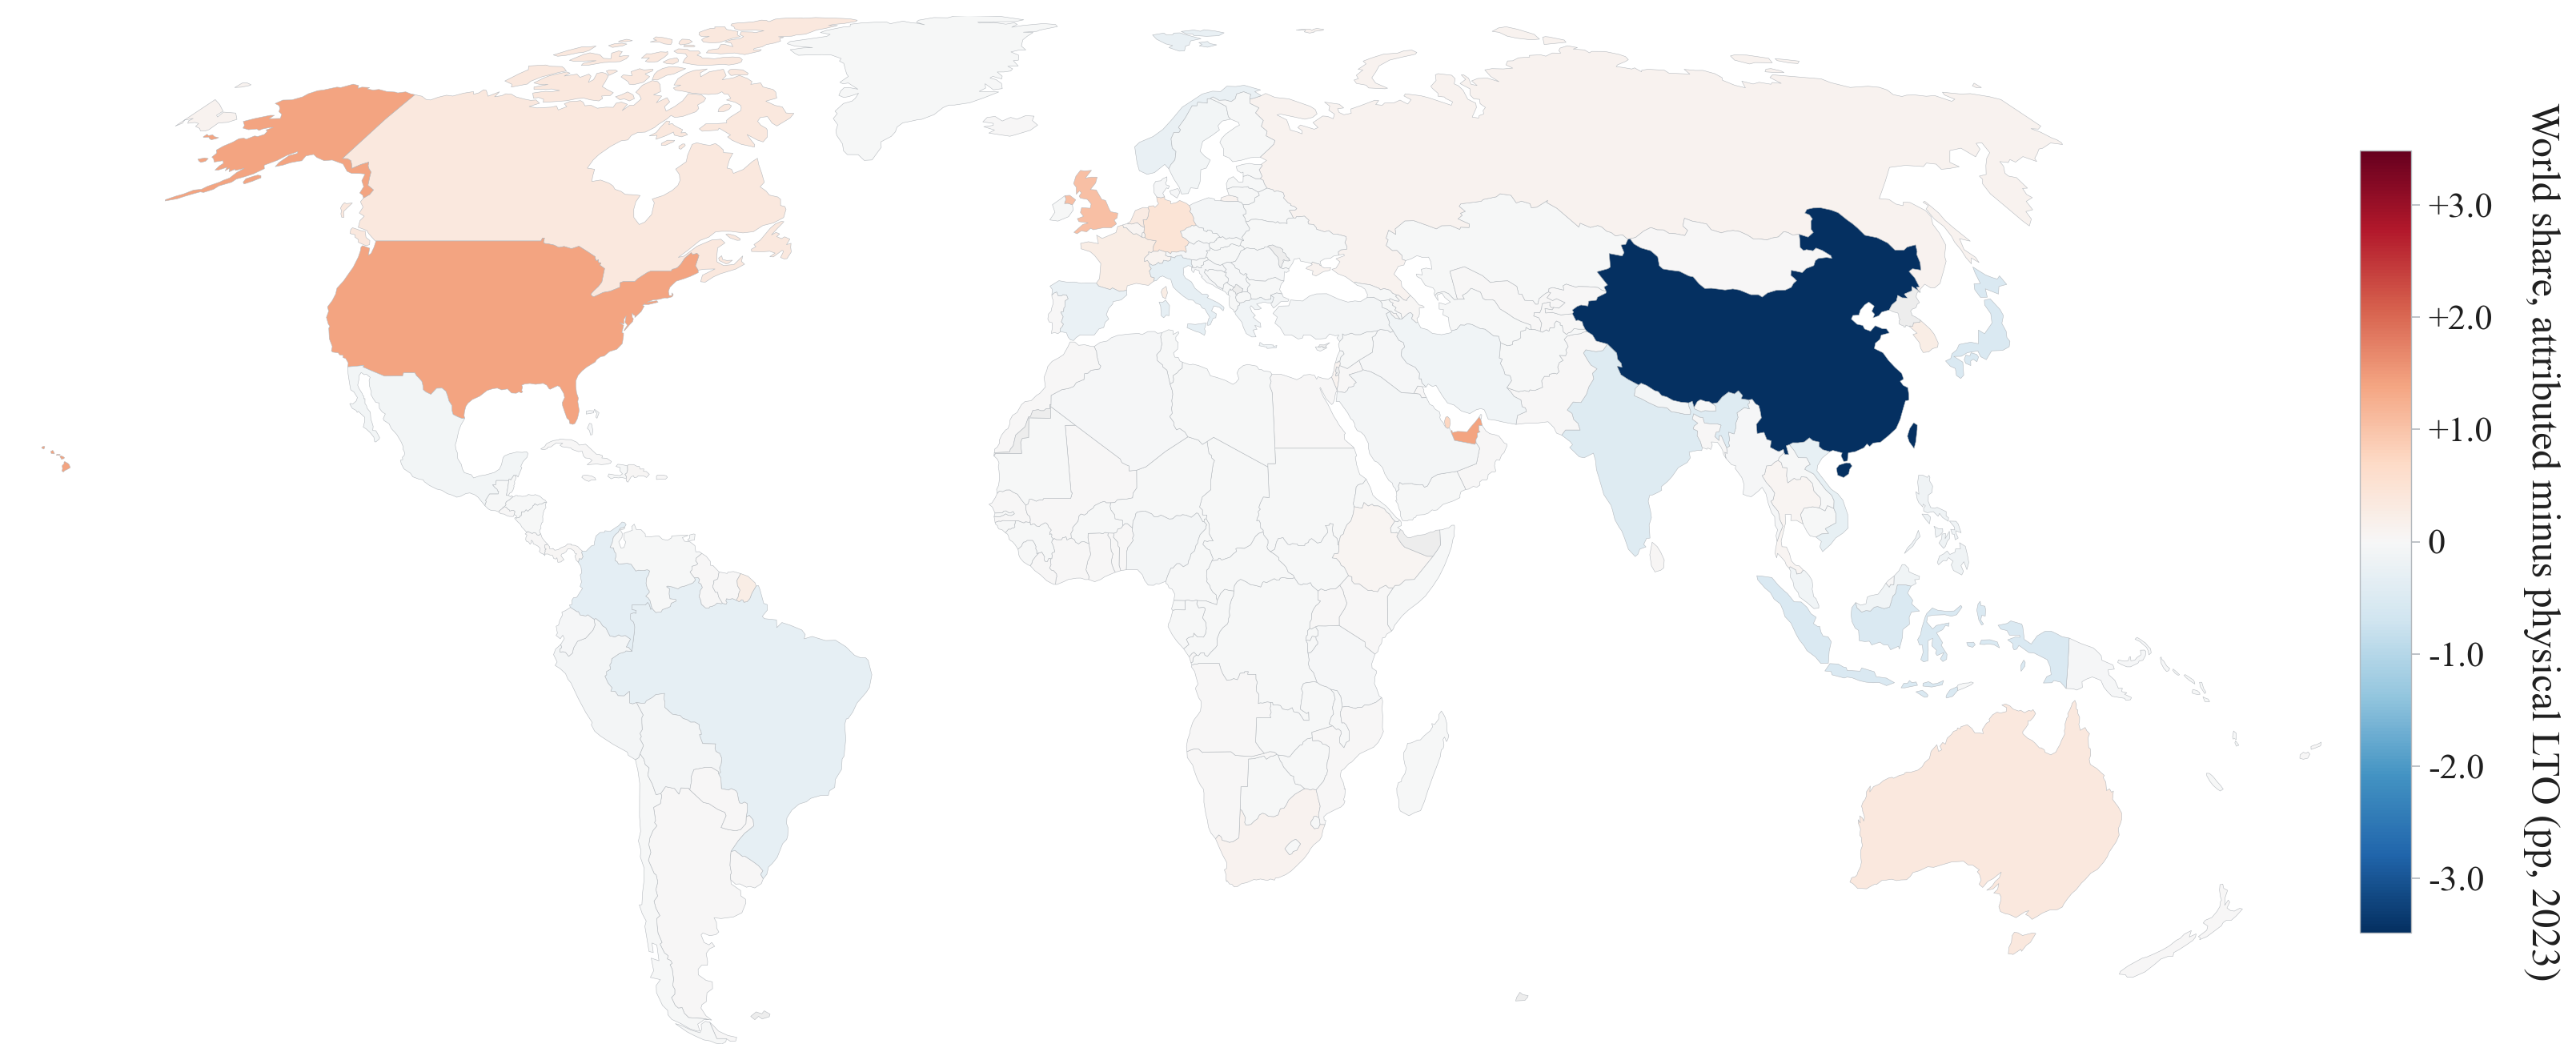
\includegraphics[width=0.92\textwidth]{CO2_map_mismatch_2023.png}
\caption{Attribution mismatch, 2023: bunker-attributed share minus physical LTO share (percentage points). Positive values indicate international hub countries; negative values indicate domestically oriented networks.}
\label{fig:mismatch}
\end{figure}

\begin{figure}[htbp]
\centering
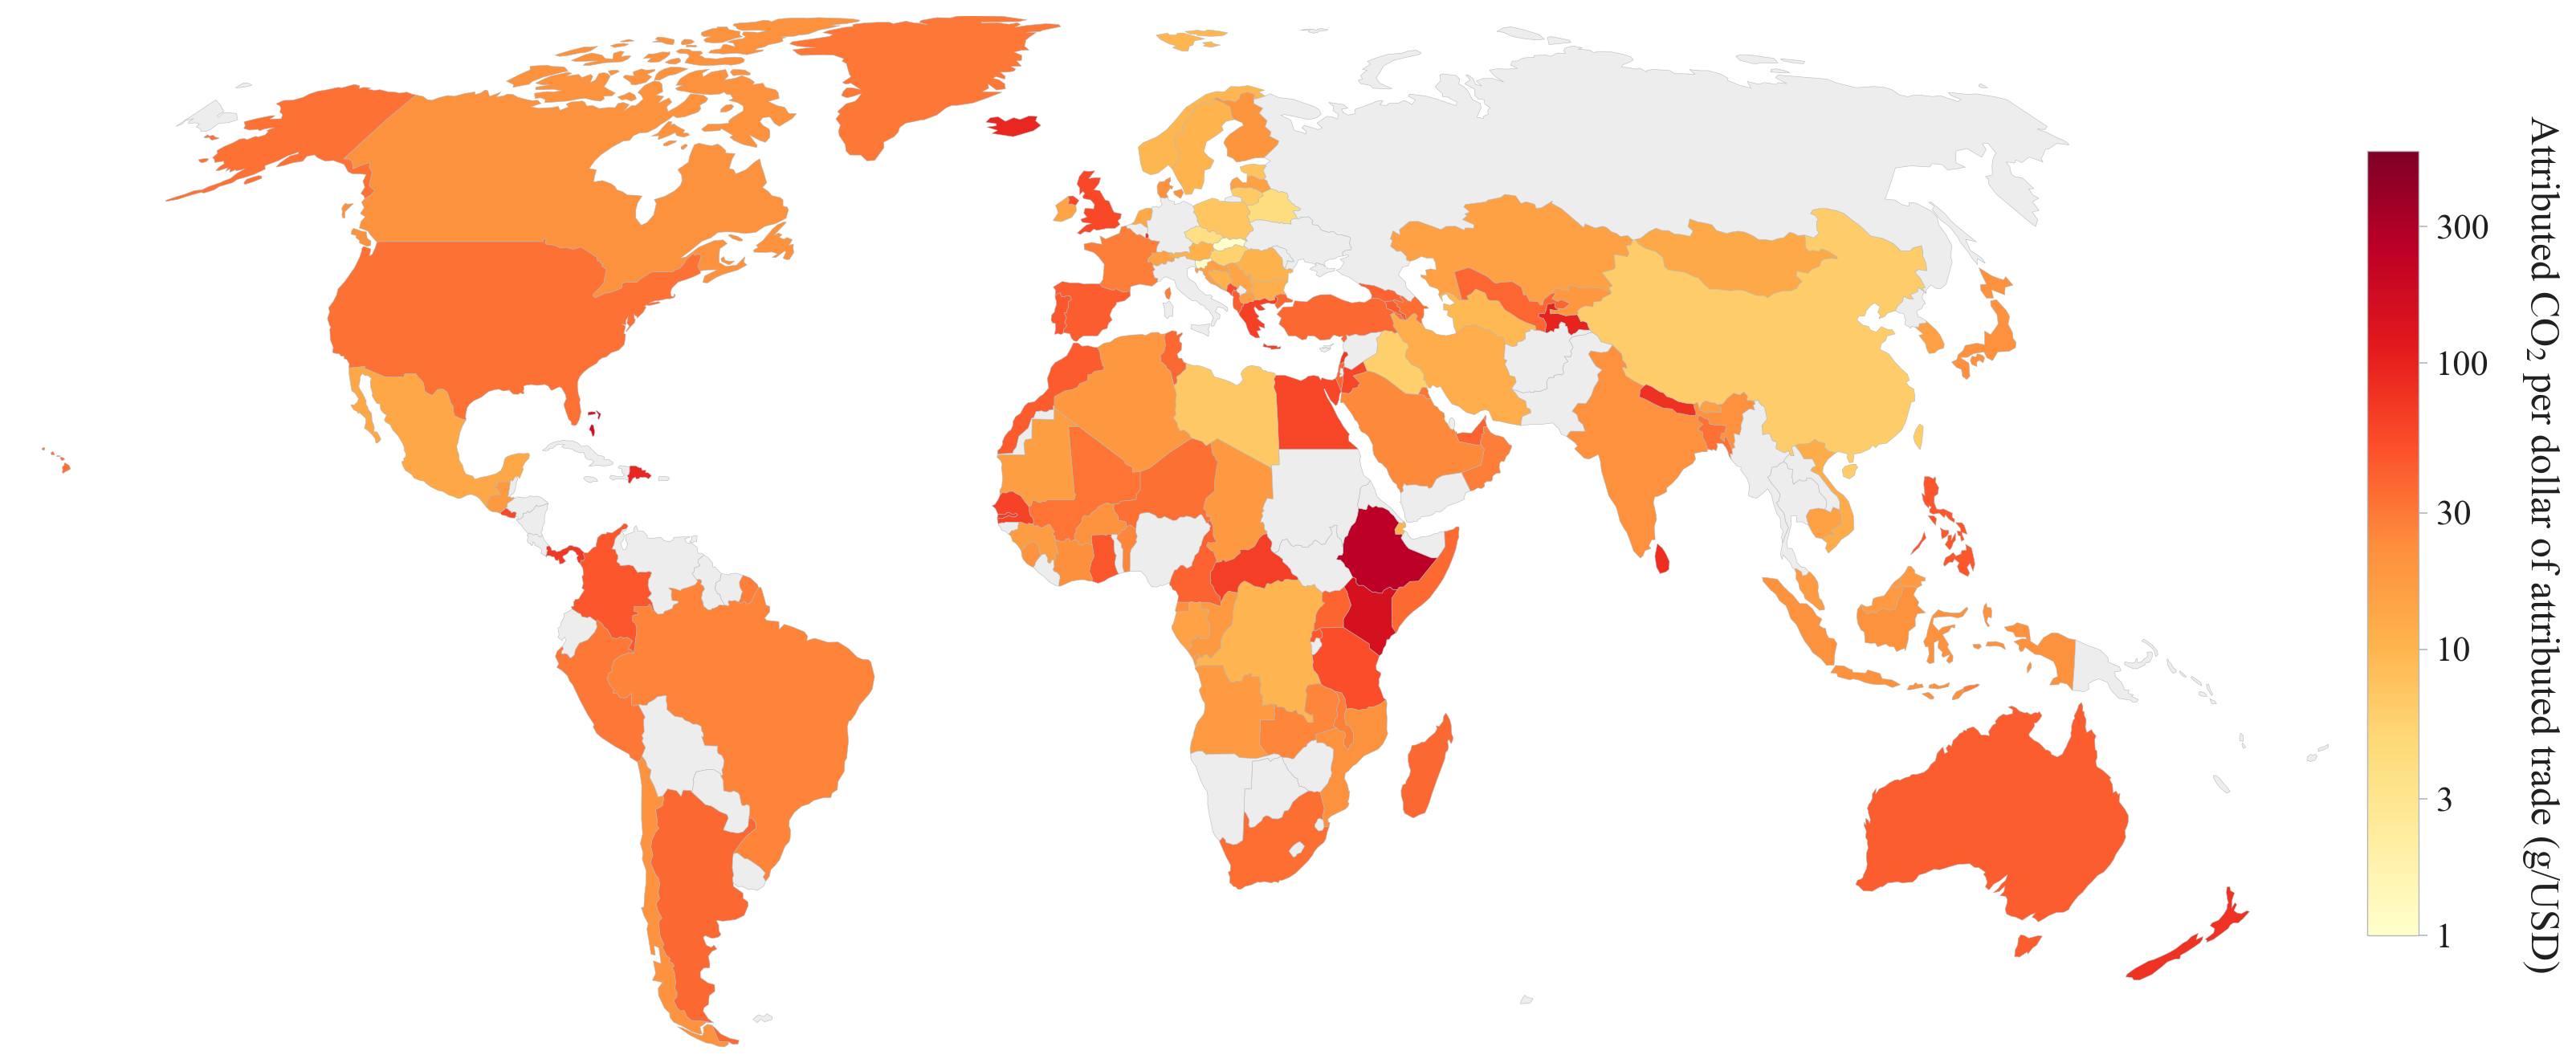
\includegraphics[width=0.92\textwidth]{CO2_map_carbonprice.png}
\caption{Carbon intensity of connectivity gains (g CO$_2$ per USD of trade gain; heritage-instrument pipeline).}
\label{fig:carbonprice}
\end{figure}

\begin{figure}[htbp]
\centering
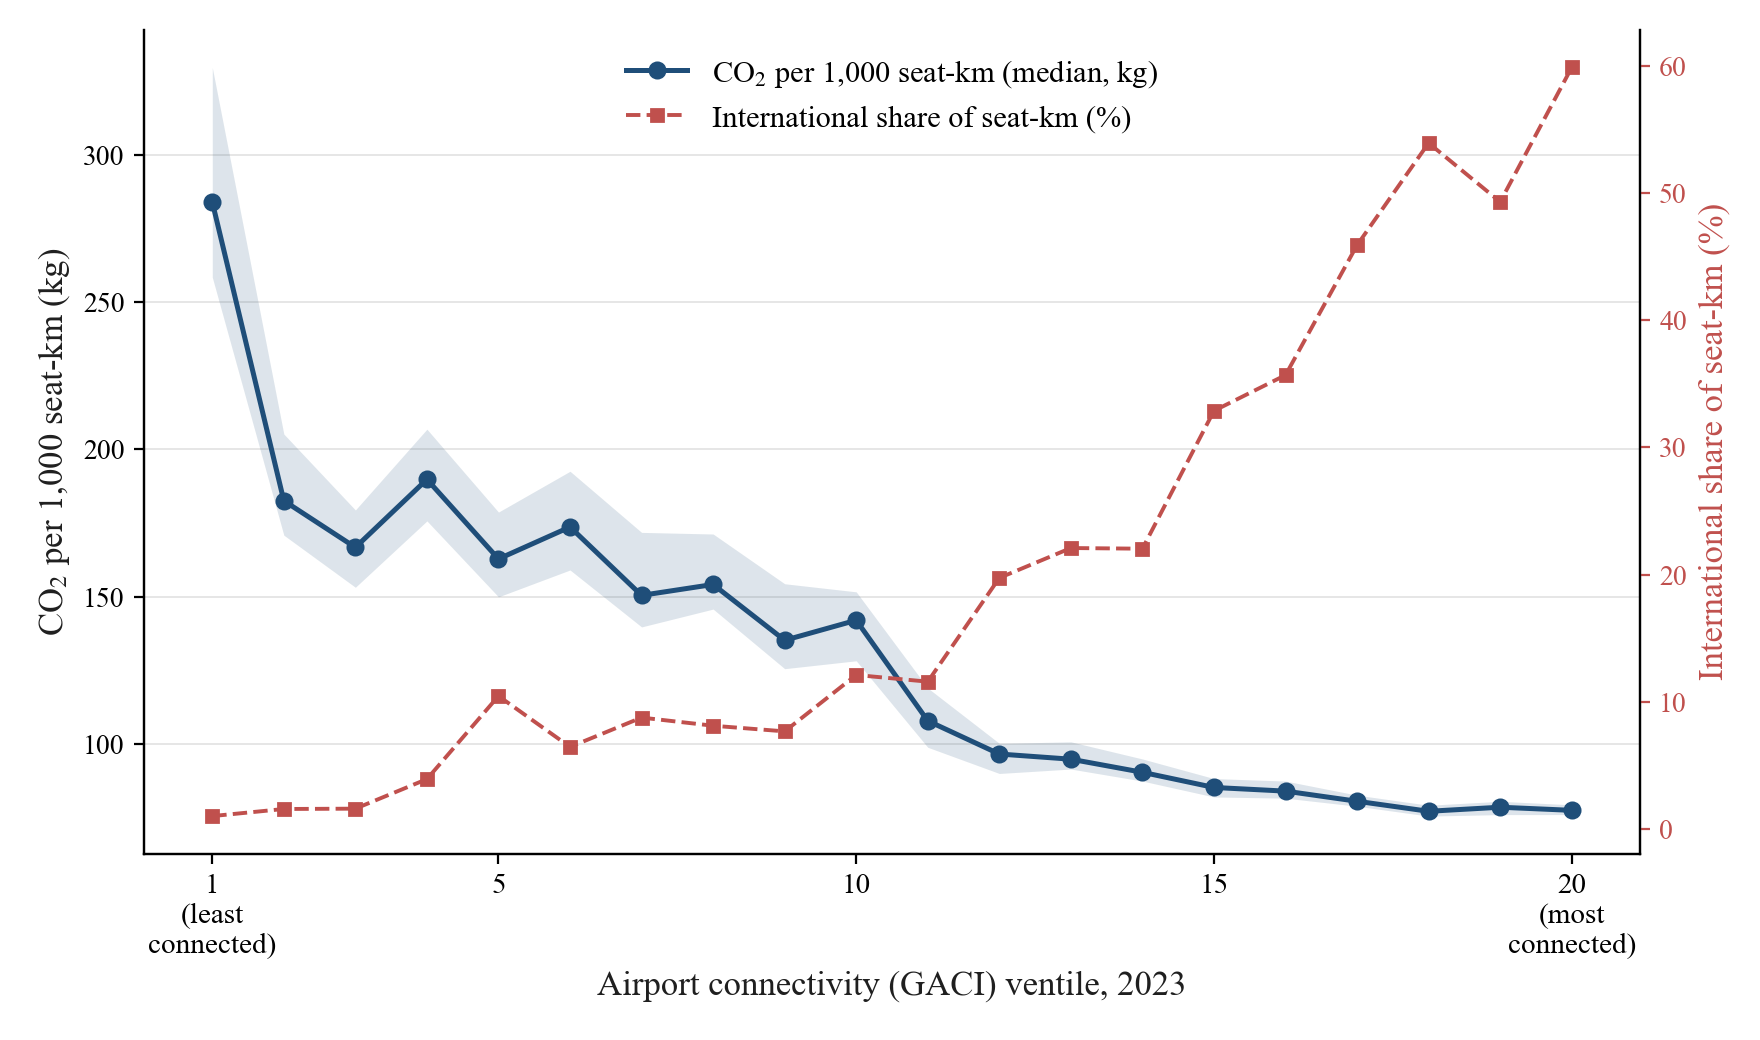
\includegraphics[width=0.92\textwidth]{CO2_efficiency_curve.png}
\caption{Airport-level efficiency curve, 2023: median kg CO$_2$ per 1{,}000 seat-km by connectivity ventile, with the international share of seat-km on the second panel.}
\label{fig:effcurve}
\end{figure}

\begin{figure}[htbp]
\centering
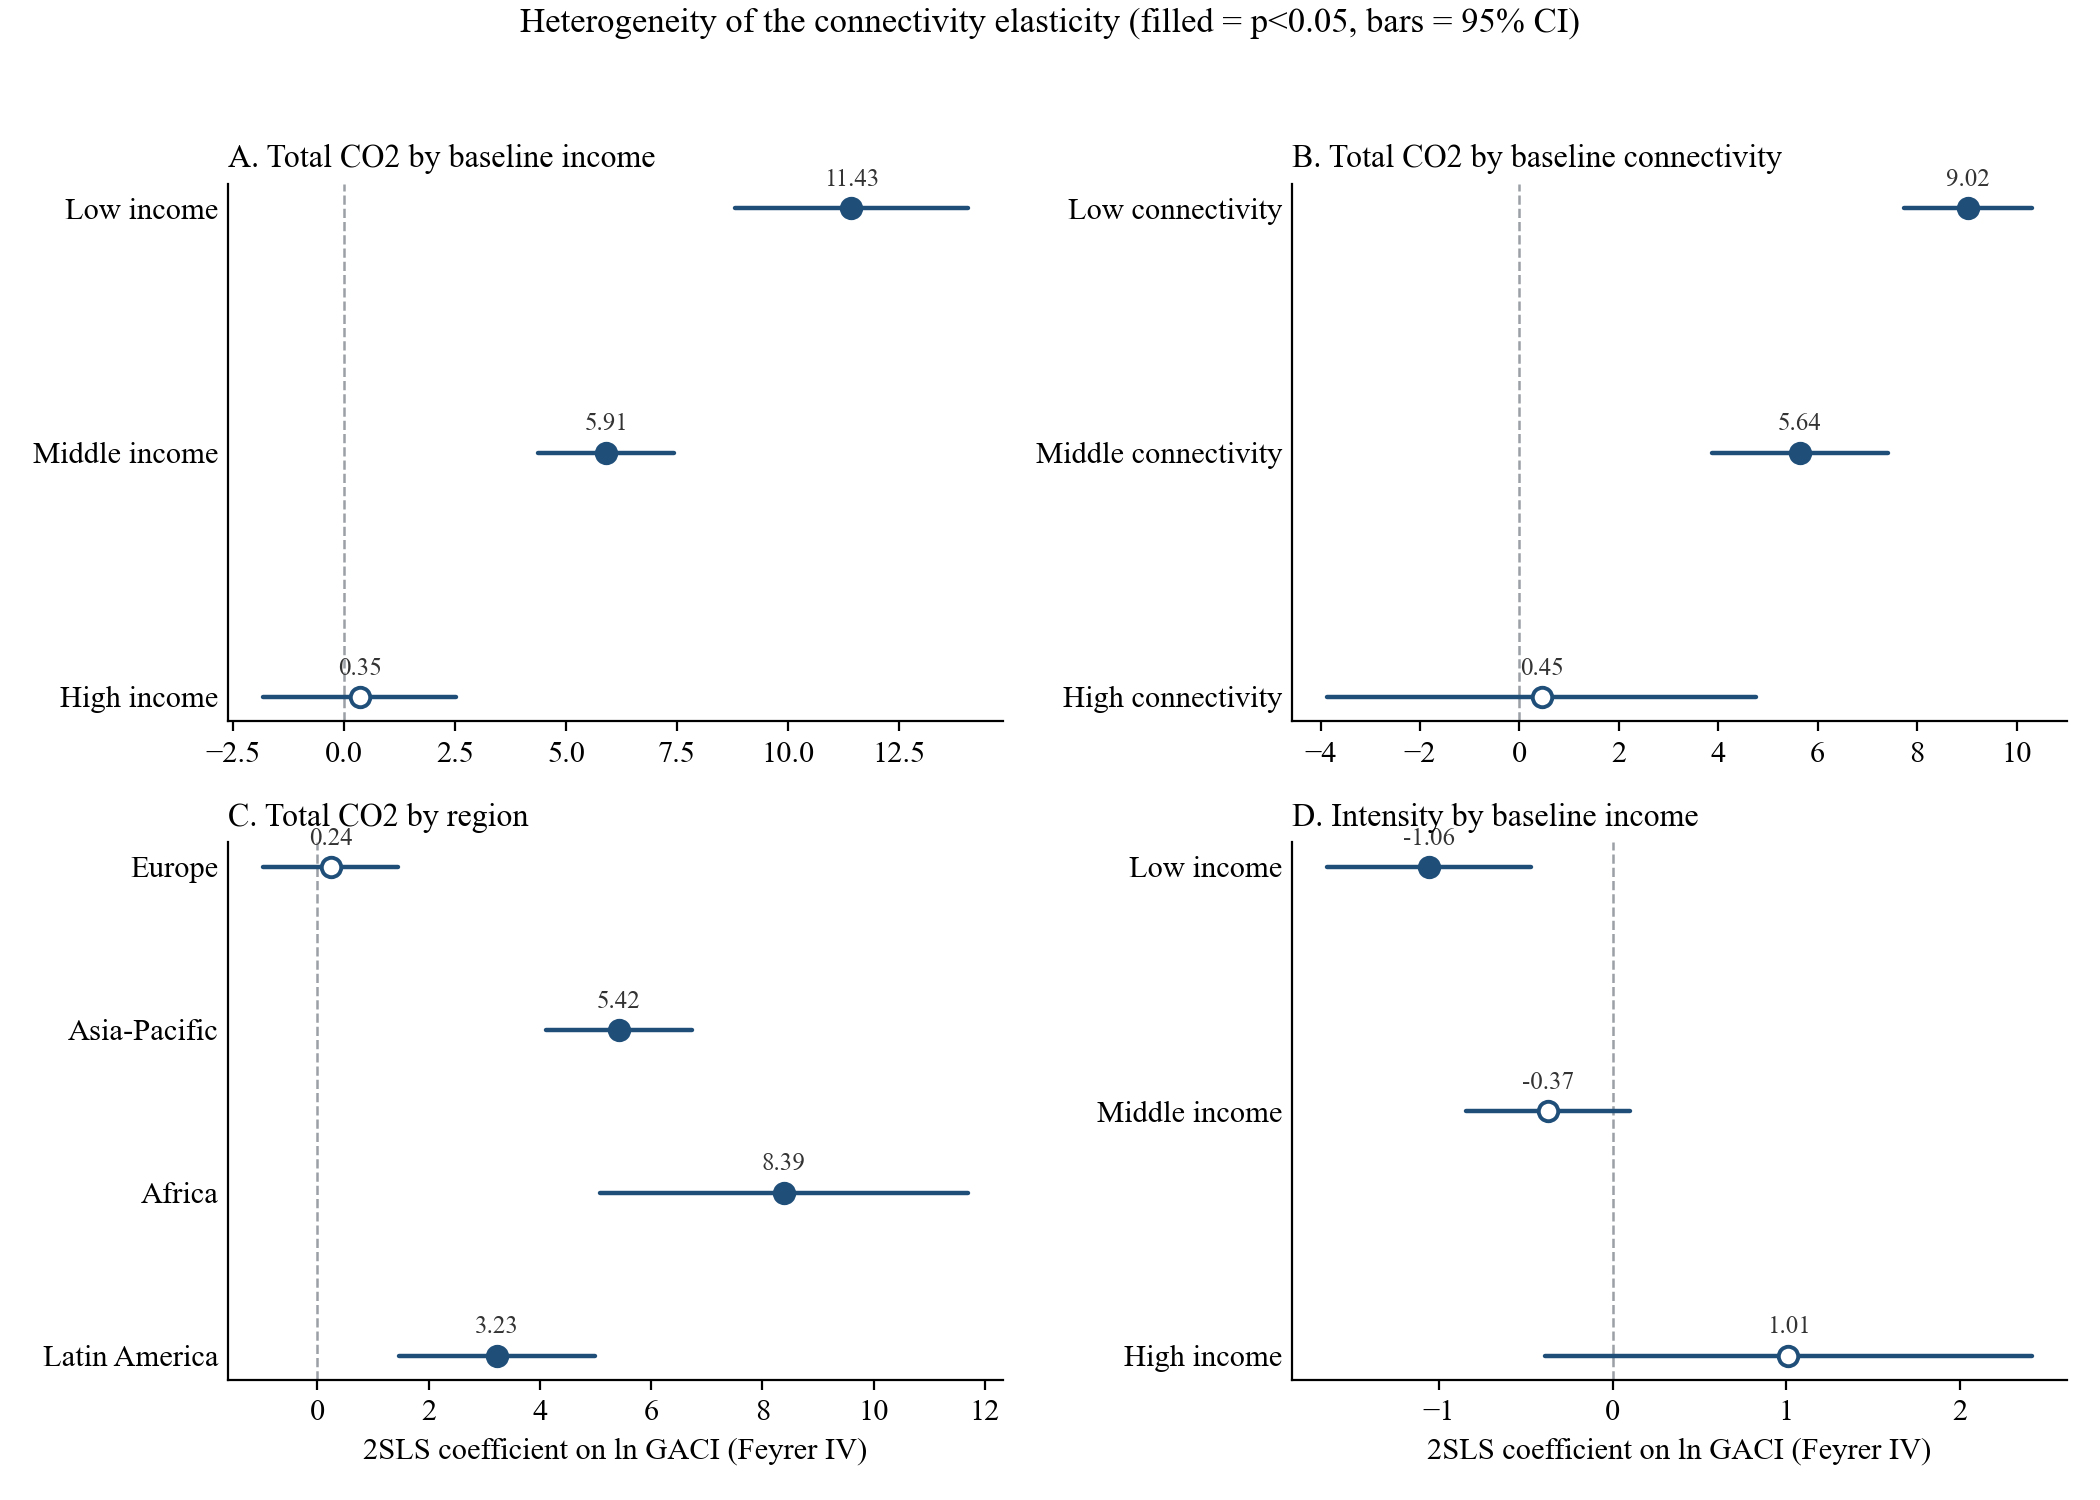
\includegraphics[width=0.92\textwidth]{CO2_hetero_coefplot.png}
\caption{Heterogeneity of the connectivity elasticity (2SLS, Feyrer instrument). Filled markers denote $p<0.05$; bars are 95 percent confidence intervals. The Middle East and North America are omitted as unidentified.}
\label{fig:hetero}
\end{figure}

\begin{figure}[htbp]
\centering
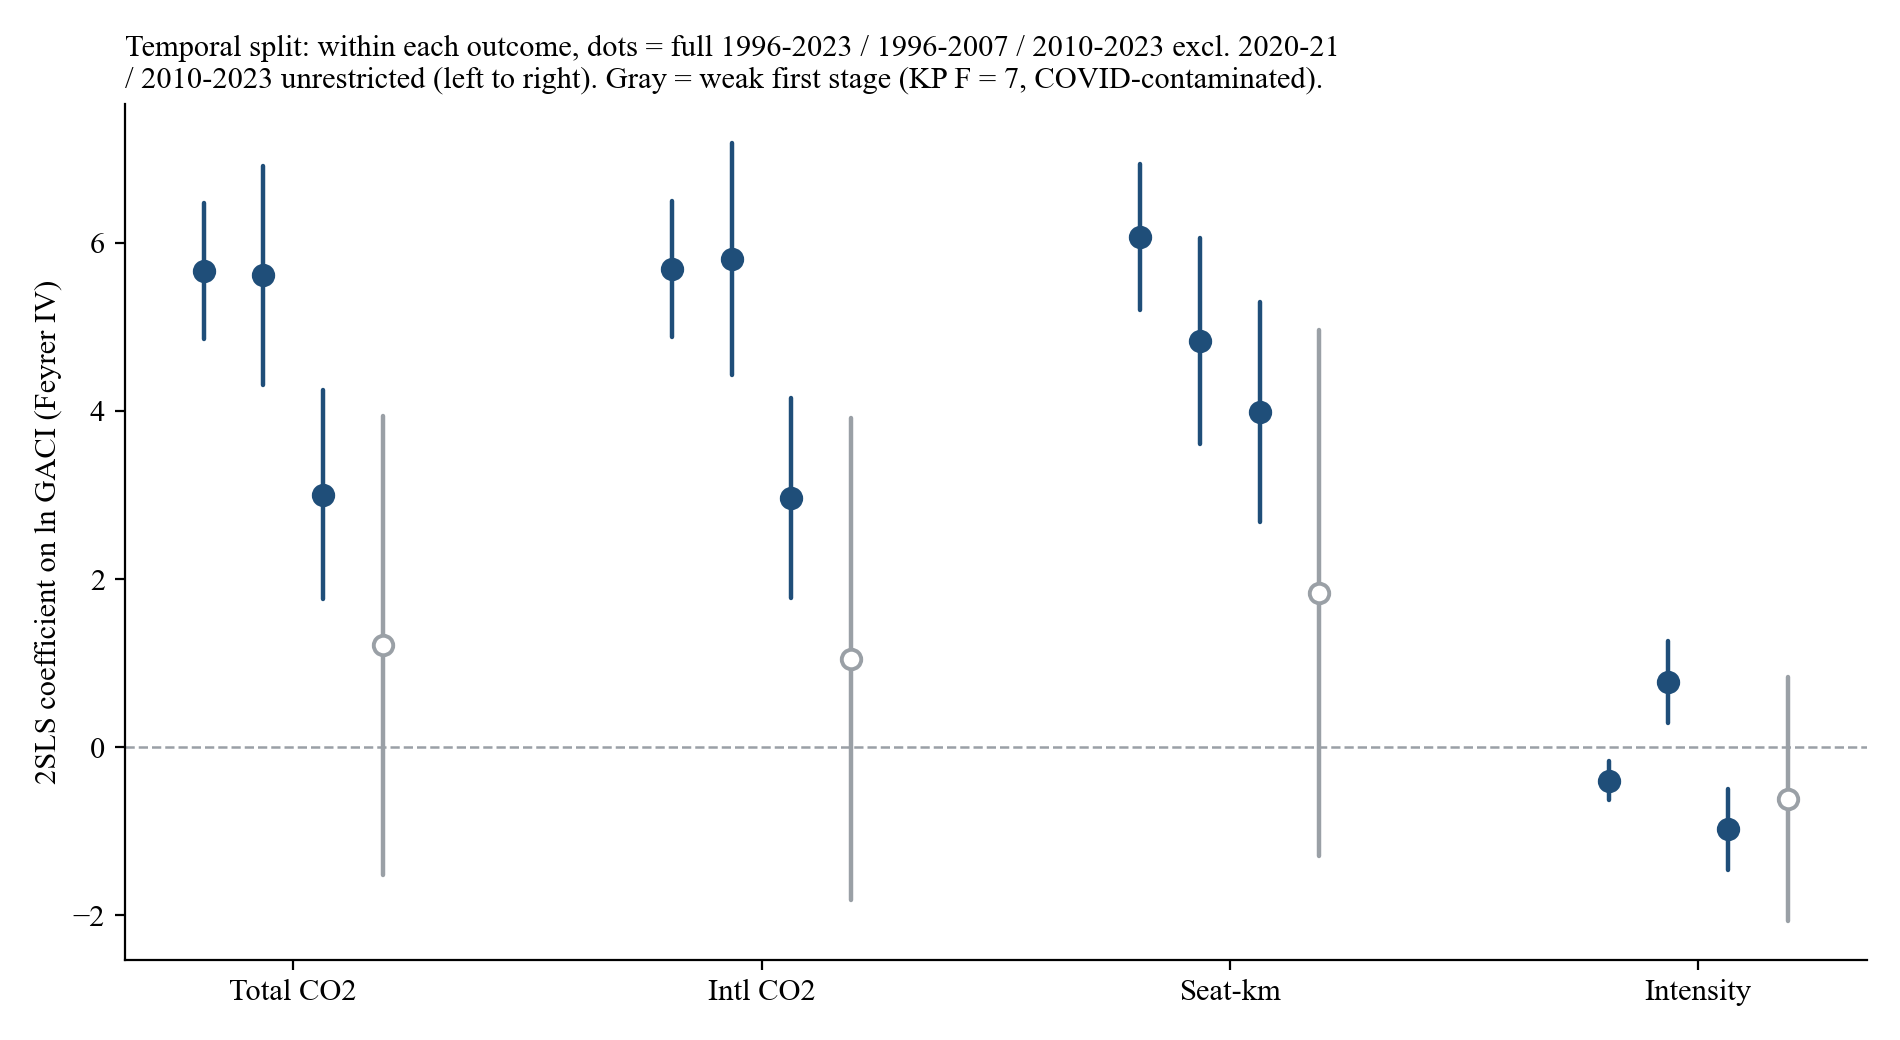
\includegraphics[width=0.92\textwidth]{CO2_temporal_coefplot.png}
\caption{Temporal split of the connectivity elasticity. Within each outcome, markers show the full sample, the network-expansion era (1996--2007), the mature-network era (2010--2023 excluding the COVID-19 years 2020--2021), and the unrestricted 2010--2023 sample from left to right; gray denotes the unrestricted later sample, whose first stage (KP $F=7$) is contaminated by the COVID collapse.}
\label{fig:temporal}
\end{figure}

\begin{figure}[htbp]
\centering
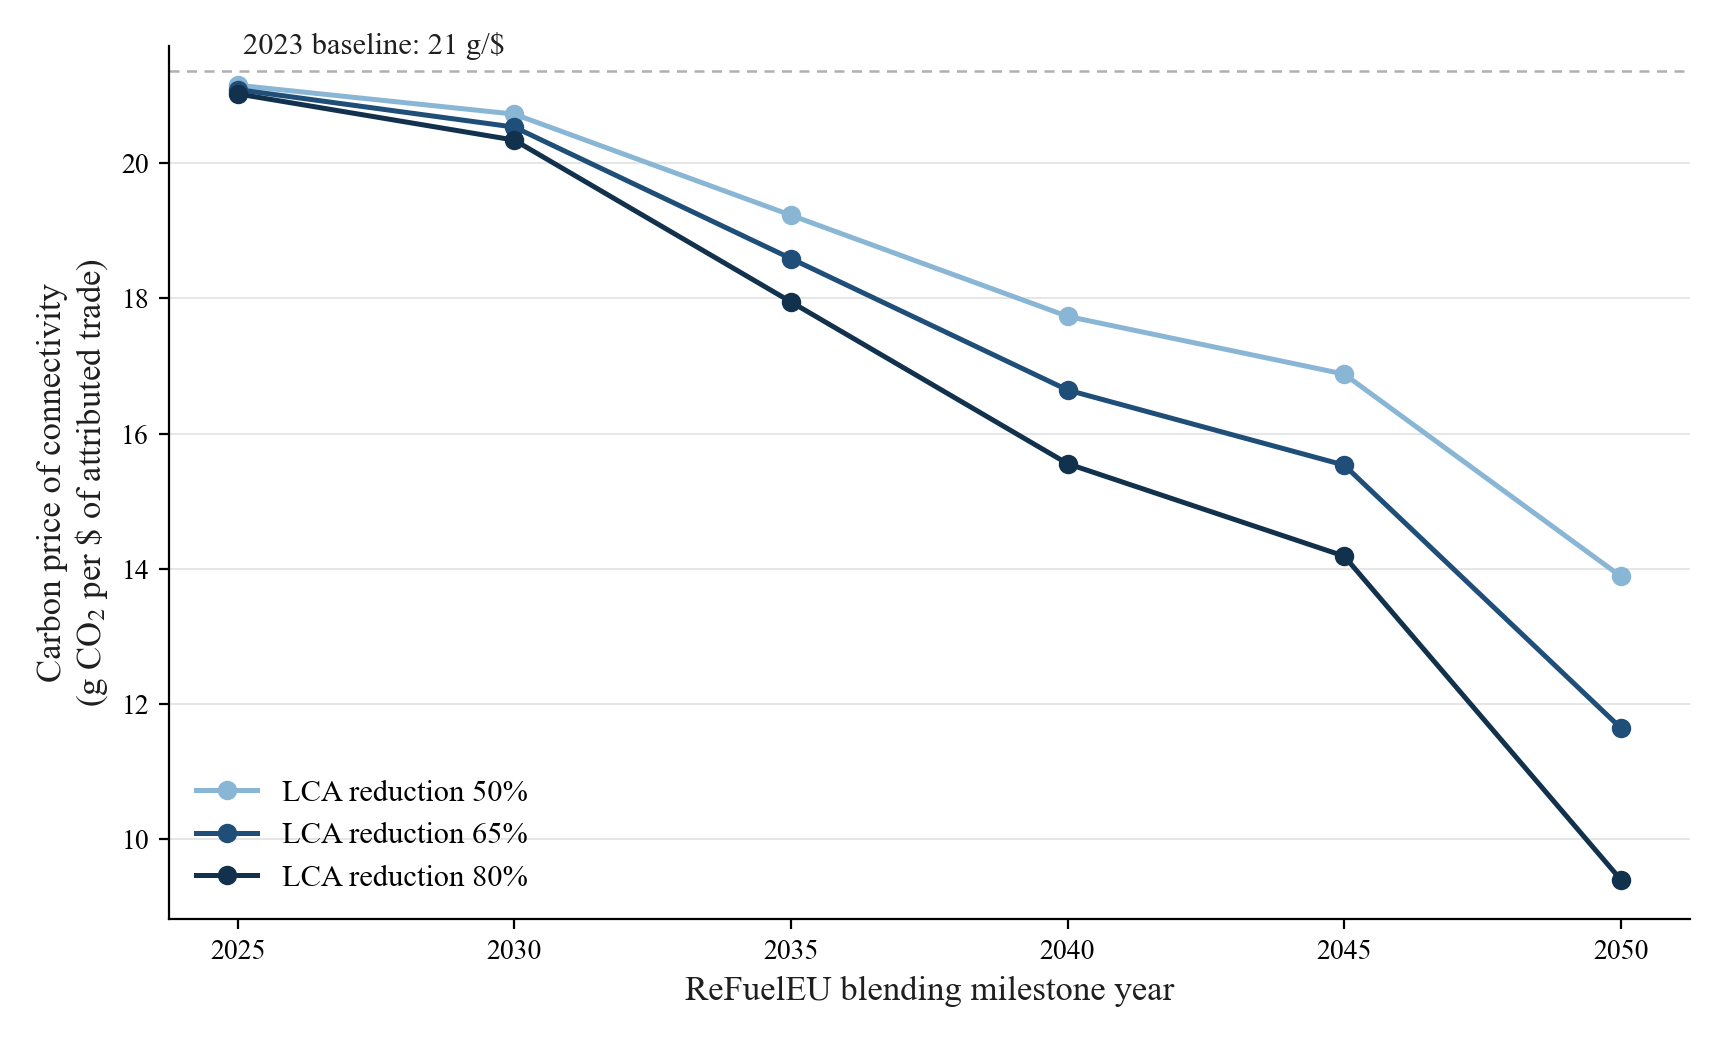
\includegraphics[width=0.92\textwidth]{CO2_saf_scenarios.png}
\caption{World aviation CO$_2$ under ReFuelEU-style SAF blending paths.}
\label{fig:saf}
\end{figure}

\begin{figure}[htbp]
\centering
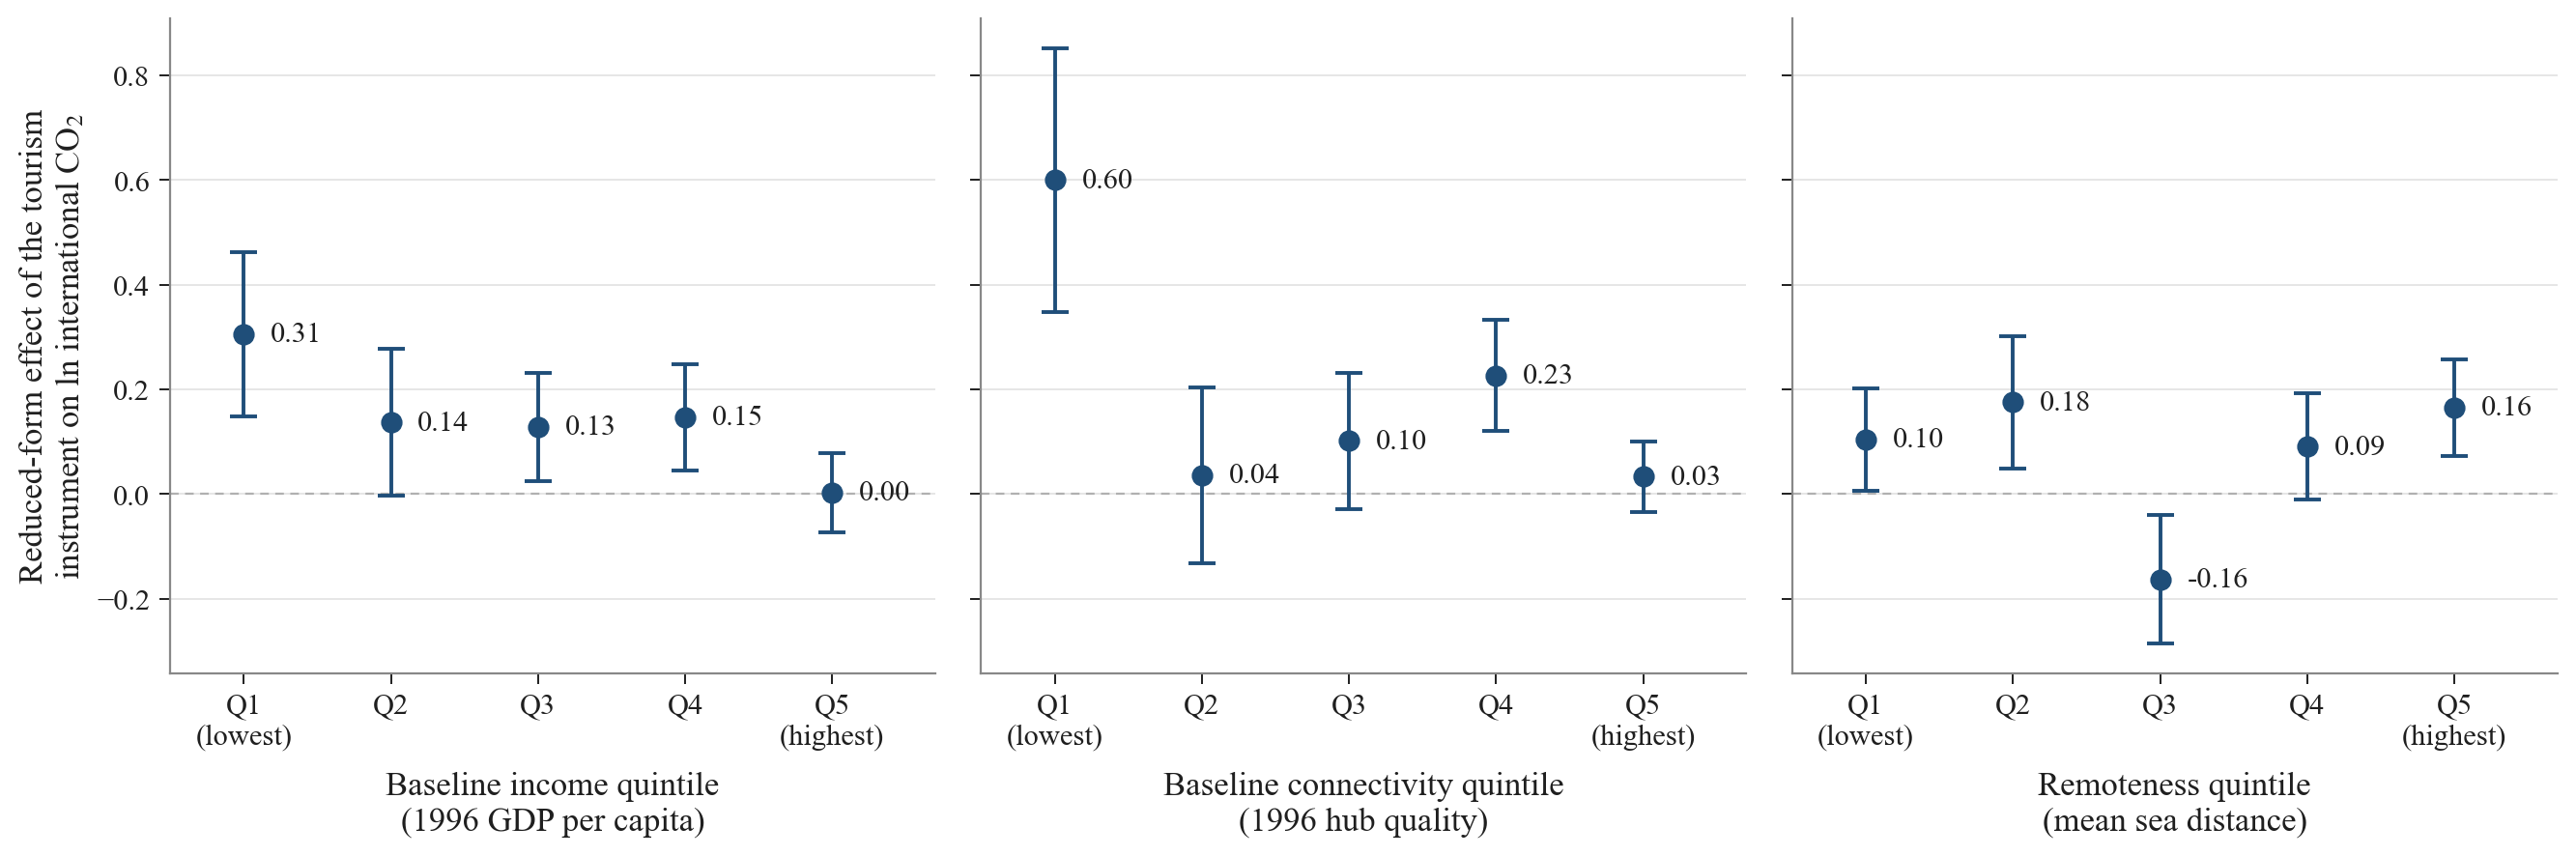
\includegraphics[width=0.92\textwidth]{CO2_rf_quintile.png}
\caption{Reduced-form quintile slopes under the tourism shifter: effects are concentrated in low-income, low-connectivity quintiles.}
\label{fig:rfquintile}
\end{figure}

\end{document}